\documentclass[a4paper,12pt]{article}
\usepackage{graphicx}
\graphicspath{ {imagesTex/} }


\begin{document}

El conjunto de nuestros datos cuenta con datos de $1917$ sujetos diferentes, para los cuales hemos elegido los cuatro \'ultimos con m\'as datos para realizar la clasificaci\'on.

Posiciones Salvador:

\begin{itemize}
\item Sujeto tetra:12082781: 41962 datos
\item Sujeto tetra:12082364: 37327 datos
\item Sujeto tetra:12086044: 28715 datos
\item Sujeto tetra:12082434: 23978 datos
\end{itemize}

Posiciones R\'io:
\begin{itemize}
\item Sujeto tetra:1121386: 12401 datos
\item Sujeto tetra:1120324: 12501 datos
\item Sujeto tetra:1131765: 12933 datos
\item Sujeto tetra:1320443: 12969 datos
\end{itemize}

\section{K-Means}

Vamos a realizar un clustering de K-medias utilizando Weka sobre el sujeto tetra:12082781; utilizando los siguientes par\'ametros:

\bigskip

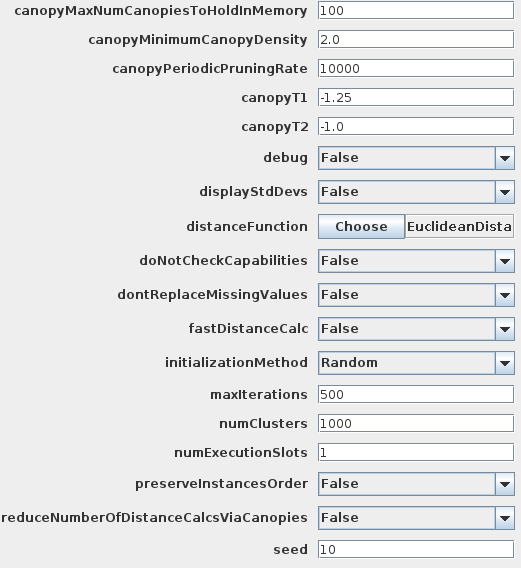
\includegraphics[scale=0.5]{kMeans_tetra:12082781.png}


Utilizamos s\'olo las variables de latitud, longitud y fecha para realizar el clustering:

Resultados: 

\section{DJ-clustering}




\end{document}